\chapter{Leggi di Moto e Profilatura delle Camme}\index{eccentrici}\index{camme}
\label{camme}

\section{Introduzione}

\noindent Nell'ambito delle macchine automatiche con elevata cadenza di funzionamento,
dedicate alla produzione su vasta scala di manufatti,
si incontrano sovente organi meccanici che eseguono movimenti ripetitivi,
composti da ben precise successioni di salite, soste e discese, nomi che tendono a essere
conservati anche quando i movimenti non sono verticali. La legge temporale di tali
movimenti \`e  solitamente
dettata dal particolare processo tecnologico che la macchina o una parte di essa
\`e chiamata a svolgere.
\begin{figure}[hbt]
\centering
\begin{minipage}[b]{0.600\textwidth}
\centering
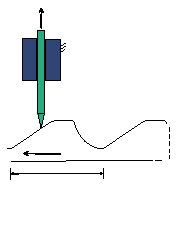
\includegraphics[width=0.9\textwidth]{part2/camme/FIG/sagoma_traslazione.pdf}
\begin{picture}(0,0)(130,5)
\scriptsize{
\put(-22,235){$y(t)$}
\put(-25,94){$v$}
\put(-15,70){$T$}
}
\end{picture}
      \caption{\em Movimentazione di un cedente mediante sagoma di traslazione.}
 \label{fig:f_sagoma_traslazione}
\end{minipage}\hfill
\begin{minipage}[b]{0.300\textwidth}
\centering
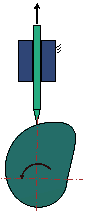
\includegraphics[width=0.9\textwidth]{part2/camme/FIG/sagoma_avvolta.pdf}
\begin{picture}(0,0)(129,0)
\scriptsize{
\put(72,220){$y(t)$}
\put(50,51) {\color{white}$\omega$}
}
\end{picture}
	\caption{\em Sagoma di traslazione avvolta su un tamburo cilindrico.}
     \label{fig:f_sagoma_avvolta}
\end{minipage}
\end{figure}
\noindent Sono frequentissimi i casi di presse e fustelle montate in cosiddette ``stazioni''
a bordo di una macchina che eseguendo particolari {\em leggi di
moto}\index{leggi di moto} tagliano, sagomano, incollano
i vari pezzi di materiale cosicch\'e, alla fine di un ``ciclo
macchina'', otterremo il manufatto finito. 
Giusto per intenderci, \`e tipico incontrare in questo perimetro
macchine automatiche  che 
producono quantit\`a elevate di stoviglie in carta o alluminio, di semplici
calzature, di tessuti, di contenitori per la cosmetica, di bottiglie
realizzate in svariate materie plastiche vuote o riempite contestualmente
alla loro formatura,
e chi pi\`u ne ha pi\`u ne metta. La cadenza di tali macchine pu\`o raggiungere e superare 
quella di due ``colpi'' al secondo.
La figura \ref{fig:f_sagoma_traslazione} riporta una idea {\em na\"ive} di un cedente 
che, tastando con una punta (o coltello) una sagoma che trasla,  viene azionato verticalmente, quindi
costretto a compiere la legge costituita dal profilo della sagoma stessa. La {\em camma lineare}\index{camme!lineari}
cos\`i ottenuta viene normalmente ``avvolta'', come in figura
\ref{fig:f_sagoma_avvolta}, su un tamburo il quale, ruotando generalmente a velocit\`a
costante, pu\`o riprodurre automaticamente ad ogni giro
la legge di moto senza la necessit\`a di ripeterla molte volte in sequenza,
come sarebbe necessario fare sulla sagoma traslante.  
\begin{wrapfigure}{r}{0.5\textwidth}
     \begin{center}
     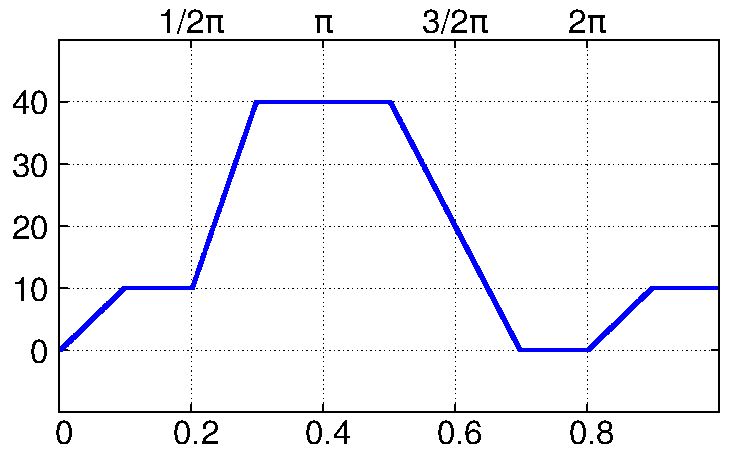
\includegraphics[width=0.42\textwidth]{part2/camme/FIG/generic_law/legge_completa.pdf}
     \end{center}
\begin{picture}(0,0)(0,0)
	\scriptsize{
	\put(155,111){$\alpha$}
	\put(6,118){$y(\alpha)$}
	\put(7,105){$y(t)$}
	\put(155,25){$t$}
	\put(130,18){$T$}
}
\end{picture}
        \caption{\em Diagramma delle alzate.}
     \label{fig:f_diagramma_alzate}
\end{wrapfigure}
\noindent Nella stragrande maggioranza delle macchine automatiche la generazione di movimenti opportuni rispettando tempi
precisi \`e di fondamentale importanza. Questo perch\'e i movimenti di fustelle,
presselli, spruzzatori, togli-metti foglio, e altri dispositivi, frequenti in 
questo ambito, necessitano di tempi e luoghi precisi per  soddisfare il processo
tecnologico al quale sono adibiti: processo che pu\`o essere rappresentato da una operazione di imbutitura, di
formatura, di incollaggio ecc. Unitamente a ci\`o, i movimenti di questi
dispositivi devono spesso 
rispettare
sincronizzazioni temporali tra le operazioni stesse e
movimenti di altri organi della medesima macchina.
Questi movimenti ripetitivi possono essere rappresentati in un grafico che prende
il nome di {\em diagramma temporale delle alzate}\index{diagramma delle alzate}, del quale un esempio \`e riportato in
figura \ref{fig:f_diagramma_alzate}.
Abbiamo poc'anzi accennato al fatto che normalmente 
la generazione delle alzate avviene tramite la trasformazione del moto
rotatorio di un albero, il quale ruota
a velocit\`a angolare  $\omega$ costante: ad ogni rotazione
completa dell'{\em albero a camme}\index{albero a camme},
sul quale sar\`a presente la {\em camma}\index{camme}, si completer\`a un intero ciclo del diagramma delle alzate.
Entreremo tra poco nel cuore di una 
descrizione, certamente non esaustiva, dei dispositivi a camma che operano la suddetta trasformazione;
anteponiamo qui solo qualche considerazione generale sulle leggi di movimento.
Tali considerazioni, peraltro, hanno applicazioni ben pi\`u estese rispetto al solo ambito delle camme meccaniche.
Riteniamo tuttavia che i meccanismi a camma offrano un generoso campo di
esempi che aiutano a comprendere l'argomento.

\section{Le Leggi di Moto}

\noindent Fissiamo le idee sulla movimentazione della mazza di una pressa
la quale dovr\`a eseguire gli spostamenti ciclici indicati
in figura \ref{fig:f_diagramma_alzate}
con una alzata massima del cedente pari
a $40\,{\rm mm}$.
Se si conviene di indicare con $T$ il {\em periodo} di tempo entro il 
quale si completa un {\em ciclo macchina}\index{ciclo macchina}, pari
nel nostro caso a $0.8\,{\rm s}$,
la velocit\`a angolare costante dell'albero che genera tale movimento sar\`a
$\omega = {2\pi \over{T}}=7.85\,{\rm rad}/{\rm s}$ che corrisponde a 75
giri al minuto.
Dato il legame tra l'angolo percorso dall'albero a camme e il tempo trascorso,
${\rm d}\alpha= \omega {\rm d}t$,  possiamo sostituire alla variabile temporale
della funzione $y(t)$ la variabile angolare $\alpha$, considerando che
in un ciclo macchina sar\`a $0 \leq \alpha \leq 2\pi$.  
Si chiama {\em diagramma delle alzate}\index{diagramma delle alzate}
il grafico di $y(\alpha)$ che mostra il legame geometrico tra le alzate di una
camma e la sua rotazione.
Si noti che la sovrapposizione del diagramma temporale delle alzate con il diagramma in funzione dell'angolo $\alpha$ \`e possibile
soltanto quando $\omega$ \`e costante, condizione questa, come abbiamo gi\`a affermato,
generalmente soddisfatta. La velocit\`a e l'accelerazione del cedente hanno
quindi un loro corrispondente di natura geometrica. Infatti derivando la 
funzione $y(t)$ rispetto al tempo otteniamo per la velocit\`a
\begin{equation}
{{\rm d}y(t)\over{{\rm d}t}}= \dot y= \omega {{\rm d}y(\alpha)\over{{\rm d}\alpha}}= \omega y'\,,
\end{equation}
\noindent e per l'accelerazione
\begin{equation}
{{\rm d}^2y(t)\over{{\rm d}t^2}}= \ddot y= \dot\omega 
{{\rm d}y(\alpha)\over{{\rm d}\alpha}}+
\omega^2 {{\rm d}^2y(\alpha)\over{{\rm d}\alpha^2}}=\dot\omega y' + \omega^2 y''\,,
\end{equation}
\noindent che, nel caso di velocit\`a angolare costante, si riduce a
\begin{equation}
\ddot y= \omega^2 y''\,.
\end{equation}
\noindent Essendo le {\em quantit\`a cinematiche geometriche}\index{velocit\`a!geometrica}\index{accelerazione!geometrica}, legate esclusivamente alla forma
della camma (pi\`u in generale legate al particolare meccanismo che le produce
utilizzando un moto rotatorio), e indipendenti dal regime di rotazione dell'albero,
esse risultano
estremamente comode per confrontare tra loro
{\em leggi di moto} diverse,
nel processo di sintesi progettuale della camma stessa.
In moltissimi casi, il diagramma delle alzate presenta una certa libert\`a interpretativa.
Spesso, ci\`o che sostanzialmente importa nella movimentazione dell'utensile
sono i valori delle successive alzate e le loro durate temporali, nonch\'e le
durate delle varie soste:
la legge di moto $y(t)$ che collega 
due posizioni di alzata invece non \`e quasi mai fissata in maniera stringente.
Nel caso del diagramma delle alzate di figura \ref{fig:f_diagramma_alzate}, ad esempio,
contiamo tre leggi di moto distinte sugli intervalli di tempo:
$0-0.1$, $0.2-0.3$ e $0.5-0.7$, frammiste a tre 
soste: $0.1-0.2$, $0.3-0.5$ e $0.7-0.8$. 
La mancanza di vincoli rigidi per i tratti di salita e discesa, cui abbiamo test\'e accennato, ci consente  la possibilit\`a di scegliere, a parit\`a
 sostanziale del
diagramma delle alzate, leggi di moto diverse che soddisfacendo tale diagramma 
possono sottostare anche ad alcuni altri criteri che sceglieremo e imporremo in
modo opportuno. Il pi\`u costrittivo di tali criteri \`e quello che permette
al cedente di giungere nei tratti di sosta effettivamente fermo. Indicando 
perci\`o con $t_s$ il tempo in cui si svolge la legge di salita deve 
essere
\begin{equation}
\int_0^{t_s} \ddot y(t) {\rm d}t=0\,.
\label{e_vel_zero}
\end{equation}
\noindent Oppure, considerando la variabile angolare anzich\'e il tempo e
indicando con $\alpha_s$ l'angolo di rotazione della camma
sul quale si estende quel tratto di salita, dovr\`a essere
\begin{equation}
\int_0^{\alpha_s}  y''(\alpha) {\rm d}\alpha=0\,.
\label{e_vel_zero_alpha}
\end{equation}
\noindent Una volta scelta la ``forma'' della
legge di accelerazione che soddisfa le relazioni \ref{e_vel_zero} e
\ref{e_vel_zero_alpha}, dovranno essere verificate le seguenti relazioni
\begin{equation}
\int_0^{t_s} {\rm d}t\int_0^{t_s} \ddot y(t) {\rm d}t\;\;=\;\;
\int_0^{\alpha_s} {\rm d}\alpha\int_0^{\alpha_s} y''(\alpha) {\rm d}\alpha=h\,,
\label{eq:ha}
\end{equation}
\noindent o anche
\begin{equation}
\int_0^{t_s} \dot y(t) {\rm d}t\;\;=\;\;
\int_0^{\alpha_s} y'(\alpha) {\rm d}\alpha=h\,,
\label{eq:hv}
\end{equation}
\noindent in maniera che tale legge produca effettivamente l'alzata richiesta.
Segnaliamo che,
nella parte dedicata agli approfondimenti, al capitolo \ref{cam2},
\`e presente 
una breve nota circa un'ulteriore propriet\`a notevole delle leggi di moto.
\vskip .3cm
\begin{figure}[hbt]
\centering
\begin{minipage}[b]{0.49\textwidth}
\centering
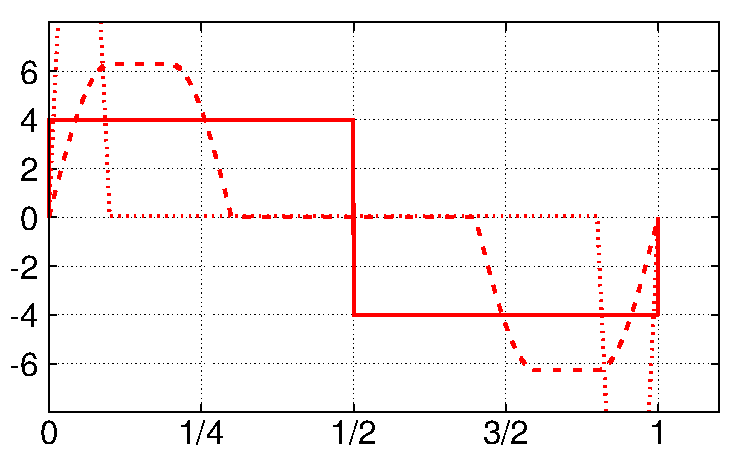
\includegraphics[width=0.9\textwidth]{part2/camme/FIG/generic_law/confronto_alzate_acc_diverse_acc.pdf}
\begin{picture}(0,0)(130,0)
\scriptsize{
\put(-20,96){${{}\ddot{y}_{3}}_{\rm max}=17.5$}
\put(-40,90){$y''$}
\put(-40,80){$\ddot y$}
\put(10,81){${{}\ddot{y}_{2}}_{\rm max}=6$}
\put(45,70){${{}\ddot{y}_{1}}_{\rm max}=4$}
\put(120,1){$\alpha$}
\put(114,1){$t,$}
}
\end{picture}
      \caption{\em Diverse leggi di accelerazione.}
 \label{fig:f_confronto_accelerazioni}
\end{minipage}\hfill
\begin{minipage}[b]{0.49\textwidth}
\centering
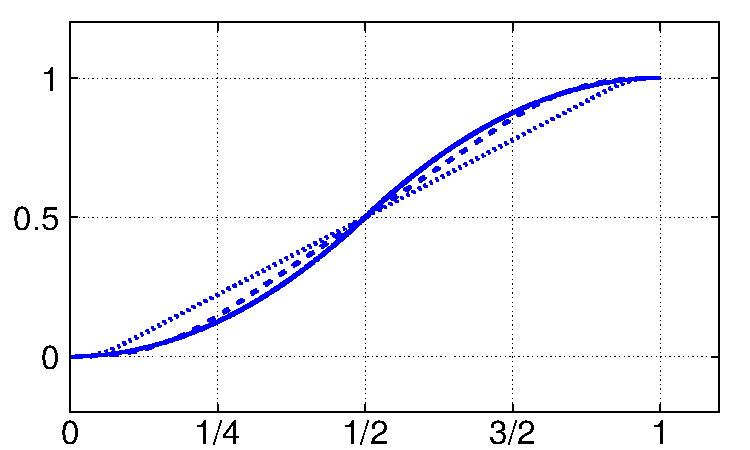
\includegraphics[width=0.9\textwidth]{part2/camme/FIG/generic_law/confronto_alzate_acc_diverse_spost.pdf}
\begin{picture}(0,0)(130,0)
	\scriptsize{
\put(-38.5,90){$y(\alpha)$}
\put(-38.5,80){$y(t)$}
\put(114,1){$t,$}
\put(120,1){$\alpha$}
}
\end{picture}
	\caption{\em Corrispondenti diagrammi dell'alzata.}
     \label{fig:f_confronto_alzate}
\end{minipage}
\end{figure}

\noindent In  figura \ref{fig:f_confronto_alzate} sono riportate tre diverse leggi
di spostamento che producono la stessa alzata, $h=1$, durante una rotazione
dell'albero di un radiante, oppure dopo il tempo di un secondo (si sottintende
perci\`o $\omega=1$), terminando la corsa con velocit\`a nulla.
Mentre la discrepanza
tra i diagrammi dello spostamento, $y(t)$ ovvero $y(\alpha)$,
risulta essere modesta, 
si pu\`o osservare che i tre diagrammi di accelerazione,
riportati in figura \ref{fig:f_confronto_accelerazioni}
unitamente ai loro valori massimi, sono molto diversi tra loro.
Ci si pu\`o chiedere: \`e sensato scegliere la
legge di moto 1) che, a parit\`a di alzata, presenta la minima accelerazione
massima? La risposta \`e s\`i e no. Infatti, il processo di sintesi
di una legge di moto per camme deve tenere conto di molte
circostanze, e la scelta di una legge che privilegi le basse accelerazioni pu\`o
presentarsi mediocre sotto altri aspetti. Cercheremo nel seguito
 di dare un 
quadro, peraltro parziale, del complesso di vincoli che guidano
la progettazione di una legge di moto e di una camma.
Riportiamo in figura \ref{fig:f_confronto_velocita}
il confronto tra le velocit\`a associate alle precedenti tre leggi di
moto in cui si nota che la velocit\`a pi\`u elevata viene raggiunta 
dalla legge con accelerazione massima minore
e viceversa.
\begin{figure}[hbt]
\centering
\begin{minipage}[b]{0.49\textwidth}
\centering
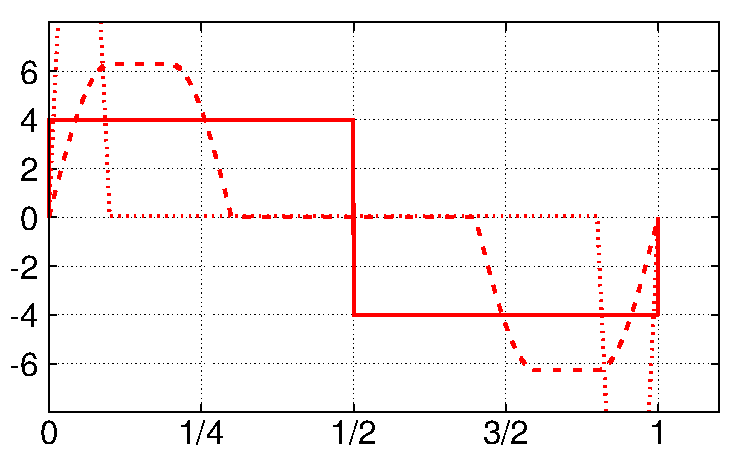
\includegraphics[width=0.9\textwidth]{part2/camme/FIG/generic_law/confronto_alzate_acc_diverse_acc.pdf}
\begin{picture}(0,0)(130,0)
\scriptsize{
\put(-20,96){${{}\ddot{y}_{3}}_{\rm max}=17.5$}
\put(-40,90){$y''$}
\put(-40,80){$\ddot y$}
\put(10,81){${{}\ddot{y}_{2}}_{\rm max}=6$}
\put(45,70){${{}\ddot{y}_{1}}_{\rm max}=4$}
\put(120,1){$\alpha$}
\put(114,1){$t,$}
}
\end{picture}
      \caption{\em Diverse leggi di accelerazione.}
 \label{fig:f_confronto_accelerazioni2}
\end{minipage}\hfill
\begin{minipage}[b]{0.49\textwidth}
\centering
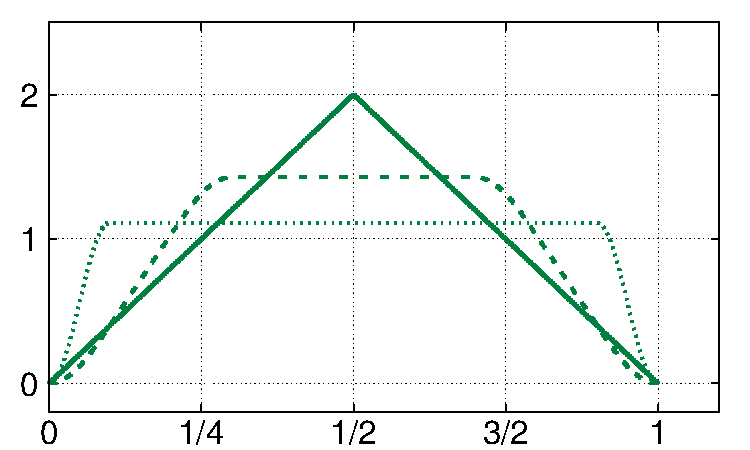
\includegraphics[width=0.9\textwidth]{part2/camme/FIG/generic_law/confronto_alzate_acc_diverse_vel.pdf}
\begin{picture}(0,0)(130,0)
\scriptsize{
\put(-48,90){$y'(\alpha)$}
\put(-48,80){$\dot y(t)$}
\put(114,1){$t,$}
\put(120,1){$\alpha$}
\put(22,80){${{}\dot{y}_{1}}_{\rm max}=2$}
\put(62,63){${{}\dot{y}_{2}}_{\rm max}=1.42$}
\put(17,39){${{}\dot{y}_{3}}_{\rm max}=1.11$}
}
\end{picture}
	\caption{\em Corrispondenti diagrammi della velocit\`a.}
     \label{fig:f_confronto_velocita}
\end{minipage}
\end{figure}

\noindent L'importanza di evitare picchi troppo elevati di accelerazione
deriva dal diretto collegamento tra questa grandezza
e l'entit\`a delle forze d'inerzia che insorgono durante il funzionamento della macchina.
Ed \`e questo il motivo che induce il progettista a disegnare la camma partendo
proprio dalle leggi di accelerazione, tenendo cos\`i sotto controllo
tale grandezza.
La legge con {\em accelerazione costante} riportata in
figura \ref{fig:f_legge_acc_cost} \`e la legge di moto pi\`u ``semplice''
che si possa adottare.
In tale figura, come nelle precedenti 
 \ref{fig:f_confronto_accelerazioni}--\ref{fig:f_confronto_velocita},
e nelle seguenti, riguardanti le leggi di moto, le ascisse riportano
sia il tempo $t$, sia l'angolo $\alpha$. Pertanto, queste leggi
possono essere qui interpretate come eseguite in un tempo unitario oppure
in un angolo unitario, ponendo cos\`i $\omega=1\; {\rm rad}/{\rm s}$. Le stesse leggi producono tutte una alzata unitaria.
\begin{figure}[hbt]
\centering
\begin{minipage}[b]{0.49\textwidth}
\centering
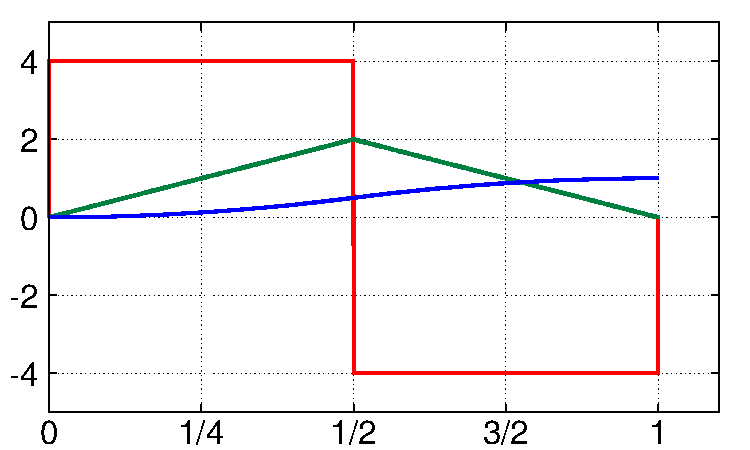
\includegraphics[width=0.9\textwidth]{part2/camme/FIG/generic_law/legge_acc_cost.pdf}
\begin{picture}(0,0)(150,-10)
\scriptsize{
\put(-17,75){$\ddot y$}
\put(-17,65){$\dot y$}
\put(-17,55){$y$}
\put(15,65){${{}\ddot{y}}_{\rm max}=4$}
\put(64,59){${{}\dot{y}}_{\rm max}=2$}
\put(140,-9){$\alpha$}
\put(134,-9){$t,$}
}
\end{picture}
\caption{\em Legge di moto con accelerazione costante.}
 \label{fig:f_legge_acc_cost}
\end{minipage}\hfill
\begin{minipage}[b]{0.49\textwidth}
\centering
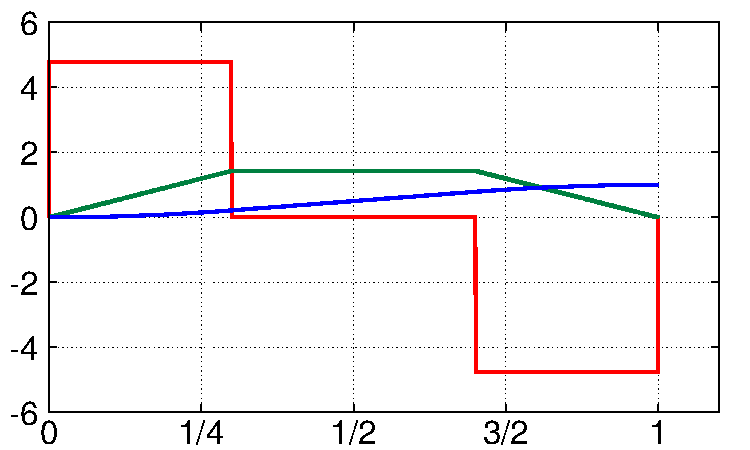
\includegraphics[width=0.9\textwidth]{part2/camme/FIG/generic_law/legge_acc_cost_tagliata.pdf}
\begin{picture}(0,0)(150,-10)
\scriptsize{
}
\put(-17,75){$\ddot y$}
\put(-17,65){$\dot y$}
\put(-17,55){$y$}
\put(39,70){${{}\ddot{y}}_{\rm max}=4.76$}
\put(48,55){${{}\dot{y}}_{\rm max}=1.43$}
\put(140,-9){$\alpha$}
\put(134,-9){$t,$}
\end{picture}
	\caption{\em Legge di moto con accelerazione costante tagliata.}
     \label{fig:f_acc_cost_tagliata}
\end{minipage}
\end{figure}
La scelta di rappresentare leggi di moto che producono
alzata unitaria in tempi o angoli unitari, leggi che chiameremo {\em unitarie}\index{leggi di moto!unitarie},
agevola il confronto
tra accelerazioni ``di forme diverse'', in quanto tale confronto
pu\`o avvenire semplicemente tra
alcuni dei valori notevoli che le grandezze cinematiche, di tali leggi
unitarie, assumono. Per passare da questi valori, cio\`e quelli
relativi alle grandezze cinematiche delle leggi unitarie e che,
limitatamente a questo capoverso, indicheremo
con pedice $u$, alle grandezze cinematiche effettive (pedice $e$) di una legge
 di uguale forma,
la quale per\`o produce un'alzata pari a $h$ in un tempo $t_s$ o in un angolo
$\alpha_s$, con riferimento agli integrali
\ref{eq:ha} e \ref{eq:hv}, si ha
\begin{equation}
\ddot y_e = \ddot y_u \frac{h}{t_s^2}\,,\;\;\;\;
{y''_e} = {y''_u} \frac{h}{\alpha_s^2}\,,\;\;\;\;
\dot y_e = \dot y_u \frac{h}{t_s}\,,\;\;\;\;
{y'_e} = {y'_u} \frac{h}{\alpha_s}\,.
\end{equation}
\noindent Ad esempio, si pu\`o notare che per la legge
ad accelerazione costante che si compie in un tempo unitario e fornisce
una alzata $h$ unitaria, si ha accelerazione massima ${{}\ddot {y}}_{\rm max}=4$,
come riportato nella figura \ref{fig:f_legge_acc_cost}.
Chiamando questa grandezza, cio\`e la massima accelerazione raggiunta
da una legge unitaria, {\em coefficiente di accelerazione}\index{coefficiente!di accelerazione} $c_a$, avremo per l'effettiva accelerazione
fornita da una legge di moto qualsivoglia
\begin{equation}
{{}\ddot{y}}_{\rm max}= c_a {h\over t_s^2}\;\;\; {\rm e}\;\;\;\;  
{{y''}}_{\rm max}= c_a {h\over \alpha_s^2}\,.  
\label{e_ca}
\end{equation}
\noindent \`E facile osservare che per una legge di moto di forma qualsiasi,
che fornisca
al suo termine $\dot {y}=0$ e che sia simmetrica rispetto alla met\`a dell'angolo sul quale si svolge, risulta $c_a \geq 4$, essendo il valore quattro
riservato proprio al caso di accelerazione costante simmetrica.
Sempre richiamando la figura \ref{fig:f_legge_acc_cost} notiamo che la velocit\`a
massima raggiunta dal cedente \`e $\dot {y}_{\rm max}=2$. Questo valore
\`e il {\em coefficiente di velocit\`a}\index{coefficiente!di velocit\`a}
 $c_v$ di questa legge di moto. 
Analogamente a quanto esposto per le accelerazioni si ha
\begin{equation}
{{}\dot{y}}_{\rm max}= c_v {h\over t_s}\;\;\; {\rm e}\;\;\;\;  
{{y'}}_{\rm max}= c_v {h\over \alpha_s}\,.  
\label{e_cv}
\end{equation}
\noindent Il coefficiente di velocit\`a, che qualifica la legge di moto rispetto
alla velocit\`a massima raggiunta, \`e altrettanto importante nella sintesi
delle camme in quanto, come vedremo tra poco, influenza direttamente
una grandezza di primaria importanza nella trasmissione del movimento.
In figura \ref{fig:f_acc_cost_tagliata} sono riportati i grafici di accelerazione
velocit\`a e spostamento per una legge cosiddetta con {\em accelerazione
costante tagliata}\index{legge!accelerazione costante} dove si nota
che, rispetto alla legge ad accelerazione costante, il coefficiente di
accelerazione cresce, mentre diminuisce quello di velocit\`a.
\begin{figure}[hbt]
\centering
\begin{minipage}[b]{0.49\textwidth}
\centering
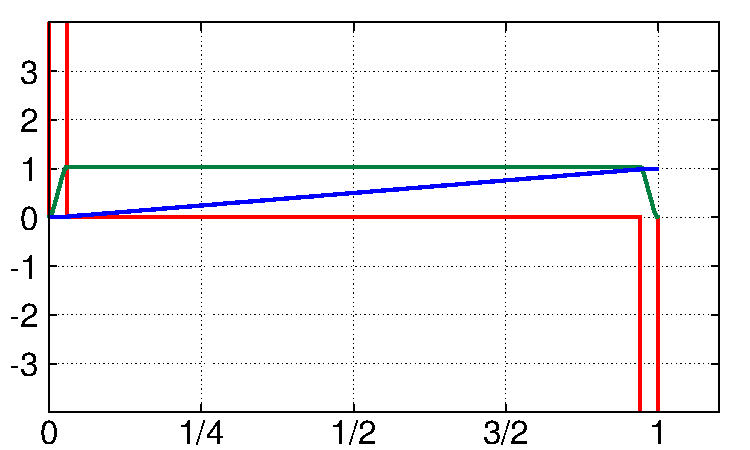
\includegraphics[width=0.9\textwidth]{part2/camme/FIG/generic_law/legge_basso_cv.pdf}
\begin{picture}(0,0)(150,-10)
\scriptsize{
}
\put(-17,75){$\ddot y$}
\put(-17,65){$\dot y$}
\put(-17,55){$y$}
\put(2,86){${{}\ddot{y}}_{\rm max}=44.9$}
\put(40,56){${{}\dot{y}}_{\rm max}=1.03$}
\put(140,-9){$\alpha$}
\put(134,-9){$t,$}
\end{picture}
      \caption{\em Legge di moto a basso coefficiente di velocit\`a.}
 \label{fig:f_legge_basso_cv}
\end{minipage}\hfill
\begin{minipage}[b]{0.49\textwidth}
\centering
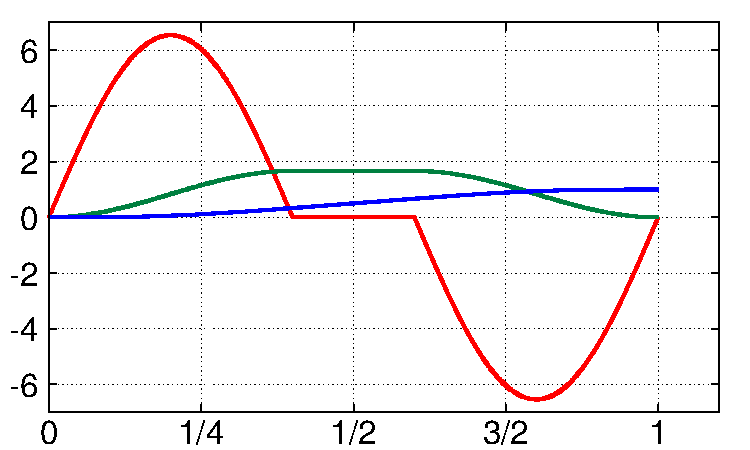
\includegraphics[width=0.9\textwidth]{part2/camme/FIG/generic_law/legge_acc_sin_tagliata.pdf}
\begin{picture}(0,0)(150,-10)
\scriptsize{
\put(-17,75){$\ddot y$}
\put(-17,65){$\dot y$}
\put(-17,55){$y$}
\put(35,74){${{}\ddot{y}}_{\rm max}=6.54$}
\put(47,56){${{}\dot{y}}_{\rm max}=1.66$}
\put(140,-9){$\alpha$}
\put(134,-9){$t,$}
}
\end{picture}
	\caption{\em Legge di moto con accelerazione sinusoidale tagliata.}
     \label{fig:f_acc_sin_tagliata}
\end{minipage}
\end{figure}
\noindent In figura \ref{fig:f_legge_basso_cv} \`e riportata una legge che presenta 
un bassissimo coefficiente di velocit\`a $c_v = 1.03$ (il limite inferiore teorico \`e uno),  
a discapito dei valori dell'accelerazione che risultano essere elevati, con
coefficiente di accelerazione $c_a=44.9$.
La legge con {\em accelerazione sinusoidale tagliata}\index{legge!accelerazione
sinusoidale} di figura \ref{fig:f_acc_sin_tagliata} soddisfa le esigenze
del progettista che \`e preoccupato delle vibrazioni che possono insorgere
durante il funzionamento della camma e che sono influenzate da cambiamenti repentini
di accelerazione: \cite{ruggieri}, pag. 45.
\begin{wrapfigure}{r}{0.5\textwidth}
     \begin{center}
     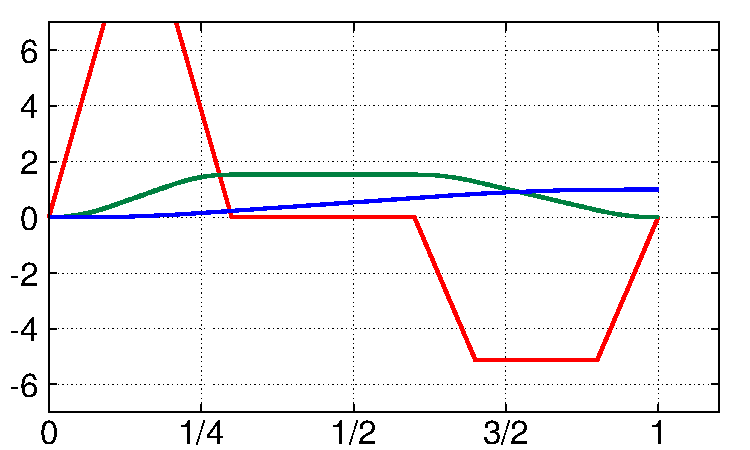
\includegraphics[width=0.42\textwidth]{part2/camme/FIG/generic_law/legge_trapezoidale.pdf}
     \end{center}
\begin{picture}(0,0)(-29,-35)
\scriptsize{
}
\put(-17,75){$\ddot y$}
\put(-17,65){$\dot y$}
\put(-17,55){$y$}
\put(-5,81){${{}\ddot{y}}_{\rm max}=7.67$}
\put(40,52){${{}\dot{y}}_{\rm max}=1.53$}
\put(129,-8){$\alpha$}
\put(123,-8){$t,$}
\end{picture}
\vskip -6mm
        \caption{\em Legge trapezoidale tagliata (asimmetrica).}
     \label{fig:f_legge_trapezoidale}
\end{wrapfigure}
\noindent La derivata terza dello spostamento,
grandezza che peraltro compare assai raramente nella meccanica, \`e in certo
modo responsabile delle vibrazioni che insorgono nella catena cinematica
del cedente durante il funzionamento delle camme veloci. La legge sinusoidale
citata poc'anzi presenta bassi valori di {\em jerk}\index{jerk} (cos\`i viene
talvolta chiamata $\dddot{y}(t)$). Purtroppo tale legge presenta, a parit\`a di
altre circostanze, valori di $c_v$ pi\`u elevati della legge ad
accelerazione costante.
\noindent In un'ottica di compromesso si potrebbe modificare la legge ad accelerazione costante rendendo le sue due ``gobbe'' di forma trapezoidale, come in figura 
\ref{fig:f_legge_trapezoidale},  passando
cos\`i da valori molto alti di {\em jerk} (teoricamente infiniti) a valori finiti
e controllabili.
Anche qui per\`o non \`e tutto rose e fiori: le rampe inclinate di questa legge di moto
si traducono in una partenza della salita poco decisa e, quel che \`e peggio,
in una difficolt\`a materiale di realizzazione in officina di queste rampe con
precisione tale da garantire l'esattezza della legge di moto
dato che, per un certo tratto, si discostano troppo poco dalla circonferenza.
\begin{figure}[t]
\centering
\begin{minipage}[b]{0.49\textwidth}
\centering
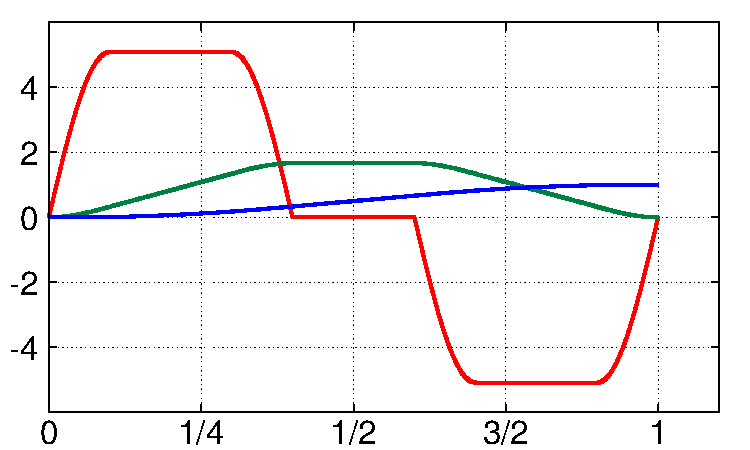
\includegraphics[width=0.9\textwidth]{part2/camme/FIG/generic_law/legge_7tratti.pdf}
\begin{picture}(0,0)(150,-10)
\scriptsize{
\put(-17,75){$\ddot y$}
\put(-17,65){$\dot y$}
\put(-17,55){$y$}
\put(43,72){${{}\ddot{y}}_{\rm max}=5.08$}
\put(48,57){${{}\dot{y}}_{\rm max}=1.66$}
\put(140,-9){$\alpha$}
\put(134,-9){$t,$}
}
\end{picture}
      \caption{\em Legge di moto con accelerazione trapezoidale modificata.}
 \label{fig:f_legge_7tratti}
\end{minipage}\hfill
\begin{minipage}[b]{0.49\textwidth}
\centering
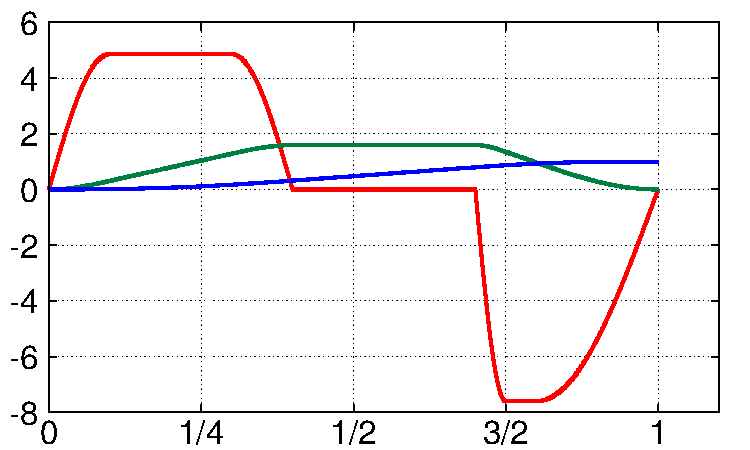
\includegraphics[width=0.9\textwidth]{part2/camme/FIG/generic_law/legge_7tratti_non_simm.pdf}
\begin{picture}(0,0)(150,-10)
\scriptsize{
\put(-17,75){$\ddot y$}
\put(-17,65){$\dot y$}
\put(-17,55){$y$}
\put(42,72){${{}\ddot{y}}_{\rm max}=4.86$}
\put(48,60){${{}\dot{y}}_{\rm max}=1.59$}
\put(38,4){${{}\ddot{y}}_{\rm min}=-7.6$}
\put(140,-9){$\alpha$}
\put(134,-9){$t,$}
}
\end{picture}
      \caption{\em Legge di moto con accelerazione asimmetrica.}
     \label{fig:f_legge_7tratti_non_sim}
\end{minipage}
\vskip -3mm
\end{figure}
\noindent Una legge di moto raffinata e spesso adottata per la sintesi delle camme, \`e senza dubbio la cosiddetta {\em legge
di moto trapezoidale modificata}\index{legge!trapezoidale modificata}, figura \ref{fig:f_legge_7tratti}.
Si compone di sette tratti: sinusoide, costante, sinusoide, nulla, sinusoide,
costante, sinusoide. Ciascuno di questi intervalli pu\`o essere lungo a
piacere permettendo in tal modo di dare origine eventualmente a leggi non simmetriche, come quella di figura \ref{fig:f_legge_7tratti_non_sim}. 

\definecolor{dark-green}{rgb}{0,0.5,0}
\begin{wrapfigure}{r}{0.6\textwidth}
\begin{center}
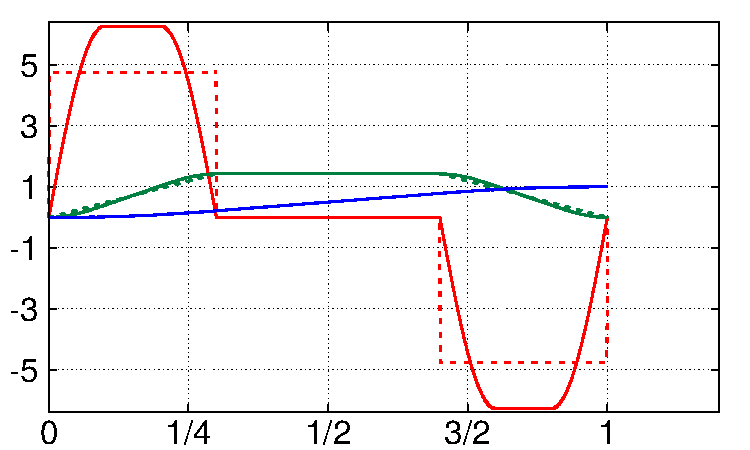
\includegraphics[width=0.55\textwidth]{part2/camme/FIG/generic_law/legge_acc_cost_e_7tratti_confronto.pdf}
\end{center}
\begin{picture}(0,0)(0,0)
\put(5,135){\color{red}$\ddot y$}
\put(5,120){\color{dark-green}$\dot y$}
\put(5,105){\color{blue}$y$}
\put(190,26){$\alpha$}
\put(184,26){$t,$}
\end{picture}
\vskip -6.5mm
      \caption{\em Confronto tra legge ad accelerazione costante e legge a sette tratti con lo stesso tempo di taglio.}
 \label{fig:f_confronto_cost_7}
\end{wrapfigure}
\noindent In figura \ref{fig:f_confronto_cost_7} si riporta,
a parit\`a di alzata e di lunghezza del ``taglio'', il confronto tra
una legge ad accelerazione costante e una legge trapezoidale modificata.
Sebbene una tale analisi
sia gi\`a stata illustrata in figura \ref{fig:f_confronto_accelerazioni},
si desidera qui esplicitarla di nuovo tramite l'impiego di due leggi molto
pi\`u usate nella pratica, in quanto la presenza del taglio assicura $c_v$
meno elevati: caratteristica, questa, molto apprezzabile, come vedremo.
\noindent Rimarchiamo ancora una volta la sostanziale equivalenza delle due leggi a livello
del diagramma delle alzate, praticamente indistinguibili nella figura.
L'inconveniente presentato dalla legge trapezoidale modificata
di avere un $c_a$ leggermente
pi\`u elevato \`e ben assorbito dalla maggiore ``dolcezza di movimento'' che essa 
garantisce.
\noindent Infine riportiamo nelle figure
\ref{fig:f_legge_completa_7_a} e
\ref{fig:f_legge_completa_7_h} rispettivamente il diagramma delle accelerazioni completo per progettare la nostra camma e il corrispondente diagramma delle alzate.
Tale diagramma, gi\`a illustrato in figura
\ref{fig:f_diagramma_alzate}, qui ottenuto per\`o
partendo da leggi di accelerazione trapezoidali modificate tagliate \`e
il candidato idoneo a essere ``avvolto'' sul tamburo della camma.
\begin{figure}[hbt]
\centering
\begin{minipage}[b]{0.49\textwidth}
\centering
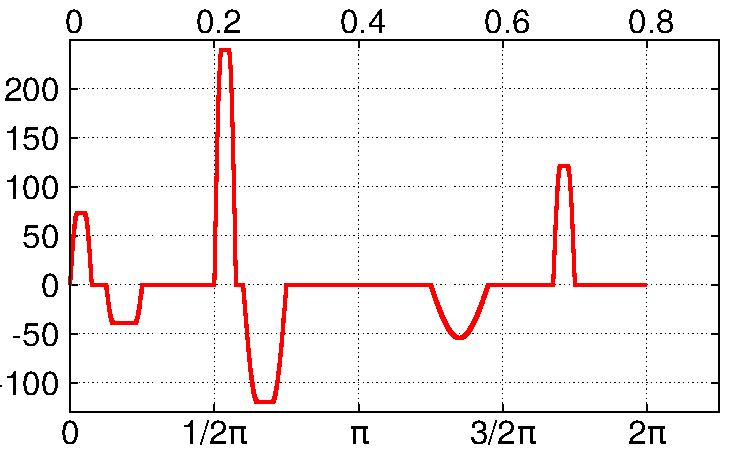
\includegraphics[width=0.9\textwidth]{part2/camme/FIG/generic_law/legge_completa_7tratti_a.pdf}
\hfill
\begin{picture}(0,0)(130,0)
\scriptsize{
\put(105,2){$\alpha$}
\put(89,97){$T$}
\put(105,89){$t$}
\put(-46,86){$y''$}
}
\end{picture}
      \caption{\em Legge completa con tratti di  accelerazione trapezoidali modificate.}
     \label{fig:f_legge_completa_7_a}
\end{minipage}
\hfill
\begin{minipage}[b]{0.49\textwidth}
\centering
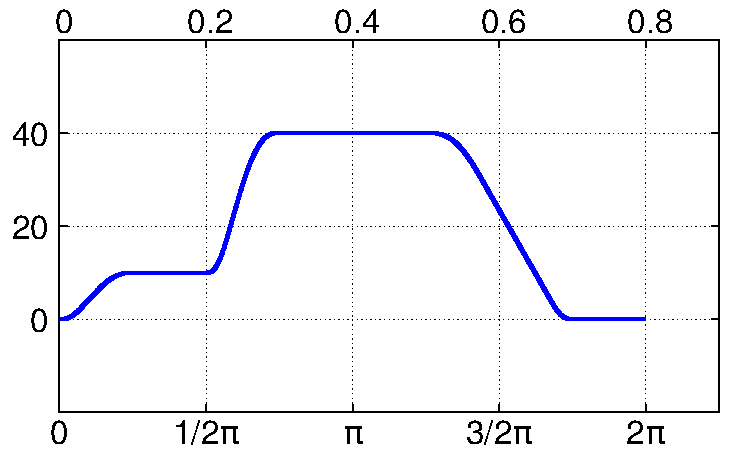
\includegraphics[width=0.9\textwidth]{part2/camme/FIG/generic_law/legge_completa_7tratti_h.pdf}
\begin{picture}(0,0)(116,0)
\scriptsize{
\put(105,2){$\alpha$}
\put(89,97){$T$}
\put(105,89){$t$}
\put(-58,86){$y(\alpha)$}
}
\end{picture}
      \caption{\em Legge completa delle alzate ottenuta da tratti di  accelerazione trapezoidali modificate.}
     \label{fig:f_legge_completa_7_h}
\end{minipage}
\end{figure}
\noindent Un'ultima considerazione circa la progettazione delle leggi di moto
dovrebbe mettere in luce la delicatezza di questo processo e l'atteggiamento
di compromesso necessario. Diamo uno sguardo alla seconda legge di accelerazione
presente nella figura \ref{fig:f_legge_completa_7_a}.
Tale legge produce in un angolo di $45^{\circ}$ un'alzata di $30\, {\rm mm}$ e,
delle tre, \`e quella con le caratteristiche pi\`u esasperate. Essa si presenta
pi\`u
``squadrata'' rispetto alle altre in modo da contenere i valori di $c_{a^+}$
(coefficiente di accelerazione considerando $\ddot y_{\rm max}$)
e di $c_{a^-}$
(coefficiente di accelerazione considerando $\ddot y_{\rm min}$). Tali valori sarebbero ancora inferiori se si eliminasse
il taglio ma questa scelta peggiorerebbe il valore dell'angolo di pressione 
$\theta$ aumentandolo e compromettendo, come vedremo a breve, il buon
funzionamento del meccanismo. 

\noindent Da un diverso punto di vista,
 contenere il valore di $c_{a^-}$ significa aumentare il valore del
minimo raggio di curvatura convessa $\rho_{\rm min}$.
Questo risulta essere un beneficio, come cercheremo di spiegare pi\`u avanti;
tuttavia,
eccedere in tal senso (aumentando il tempo su cui si estende la ``gobba''
negativa dell'accelerazione) produrrebbe il pessimo risultato di
aumentare $c_{a^+}$, parametro che governa
le forze d'inerzia durante l'alzata.

\vskip 1mm
\null
\section{Profilatura delle Camme}\index{camme}

\noindent Come accennato all'inizio di questo capitolo, la legge di spostamento
$y(\alpha)$ 
viene (salvo casi particolari) avvolta su di un tamburo in modo da generare
una camma piana.
Nel processo di sintesi della camma le grandezze  in gioco sono molte e tra
queste il raggio del tamburo test\'e citato, che si chiama {\em raggio di base}\index{raggio
di base} e che verr\`a indicato con $R_b$, gioca il  ruolo pi\`u importante.
All'aumentare del raggio di base scompaiono infatti dalla
camma le problematiche principali di profilatura,
cui accenneremo fra poco.  Di contro,  col crescere di $R_b$,
aumentano le dimensioni della camma stessa rendendola 
scomoda da utilizzare nel progetto organico di una macchina\footnote{Ci preme
precisare 
che il raggio di base pu\`o essere riferito a entit\`a geometriche diverse
dal profilo fisico della camma. In particolare, vedremo che le camme tastate
da una rotella presentano un importantissimo luogo geometrico ``virtuale'', il
{\em profilo del
centro rotella}, che coincide con il profilo di una camma tastata da una punta che esegue le stesse leggi di moto.
In questo caso $R_b$ sar\`a il raggio della circonferenza minima
tangente al tracciato del centro rotella, in quanto difficilmente
risulter\`a utile tirare in ballo il raggio di base del profilo fisico.
Pertanto, nonostante
molteplici trattazioni pi\`u autorevoli della nostra introducano per
il raggio di base del profilo del centro rotella  il simbolo $R_{b0}$, siamo convinti
di non creare equivoci accontentandoci di usare soltanto $R_b$.
}.
Si intravede quindi un percorso di progetto 
che ha come obiettivo quello di trovare una soluzione
che, evitando eventuali criticit\`a 
derivanti da dimensioni geometriche mal scelte (quasi sempre
valore di $R_b$ insufficiente),
soddisfino anche requisiti di compattezza, limitazione
dell'ingombro
 e funzionalit\`a.
La figura \ref{fig:f_ang_press} ci aiuta a riconoscere una delle grandezze
geometriche 
fondamentali di un meccanismo a camma: l'{\em angolo di pressione} $\theta(
\alpha)$, funzione i cui valori, in generale,
variano nell'arco dell'angolo giro.
Notiamo subito che $\theta$ \`e anche l'angolo compreso tra la retta tangente al
profilo nel punto di contatto col cedente e una retta generica
ortogonale al cedente stesso. 
\begin{figure}[bht]
\centering
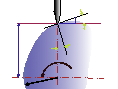
\includegraphics[width=0.8\textwidth]{part2/camme/FIG/ang_press.pdf}
\begin{picture}(70,0)(130,0)
\scriptsize{
\put(222,202){$\theta$}
\put(208,183.5){${\rm d}y$}
\put(168,167){${\rm d}\alpha (R_b+y)$}
\put(168,111){$\theta$}
\put(55,99){\rotatebox{90}{{$R_b + y$}}}
\put(150,82){$\omega$}
\put(100,33){$R_b$}
}
\end{picture}
      \caption{\em Angolo di pressione $\theta$.}
 \label{fig:f_ang_press}
\end{figure}
La forza $F$  che la camma deve trasmettere al cedente,
soggetto a una spinta assiale $S$, risulta
essere $F=S/\cos(\theta)$, relazione dalla quale si evince l'importanza
di mantenere l'angolo $\theta$ entro stretti limiti.
Angoli $\theta > 30^{\circ}-35^{\circ}$ non sono
in genere accettabili nei tratti di salita, dove cio\`e la camma spinge la
punteria, riservando il valore limite pi\`u elevato a soluzioni
che prevedono guide di scorrimento per la punteria con attriti particolarmente
ridotti, \cite{molian}, pagg. 131-132. \`E frequente, nell'ambito delle macchine
automatiche, l'utilizzo di punterie costituite da colonne 
a sezione circolare, rettificate, che scorrono in manicotti a ricircolo di
sfere con attrito molto limitato.
Pertanto poniamo il massimo angolo di
pressione tollerato al valore $\theta_{\rm lim}=35^{\circ}$, osservando che angoli
di pressione maggiori genererebbero una forza ortogonale al cedente troppo
elevata col pericolo di impuntamento di quest'ultimo, oppure di una trasmissione
del movimento poco efficiente.
Poniamoci dal punto di vista relativo a un osservatore solidale con la camma.
In tale riferimento la punta percorrer\`a, durante una rotazione infinitesima
${\rm d}\alpha$ dell'albero, un tratto infinitesimo della tangente nel punto di contatto.
Questo tratto infinitesimo si scompone facilmente sui cateti 
del triangolo rettangolo
${\rm d}y$ e ${\rm d}\alpha (R_b +y)$, dalla quale scomposizione risulta
\begin{equation}
\tan(\theta)={{\rm d}y\over{(R_b+y)}{\rm d}\alpha}= {y'\over{R_b+y}}\,.
\label{e_ang_press}
\end{equation}
\noindent Affinch\'e il meccanismo funzioni correttamente il valore massimo di questa espressione dovr\`a essere contenuto al di
sotto del valore prescritto. Purtroppo \`e alquanto probabile che il massimo valore di $y'(\alpha)$ e il minimo di $y(\alpha)$ non si verifichino per lo
stesso angolo $\alpha$, quindi 
occorrerebbe cercare il massimo della funzione \ref{e_ang_press}. 
\noindent Ricordiamo che $y'_{\rm max}=c_v h/\alpha_s$, cio\`e il massimo
valore della velocit\`a geometrica \`e dato dal coefficiente di velocit\`a
della legge di moto moltiplicato per l'alzata e diviso per l'angolo di salita.
In via cautelativa si pu\`o asserire che affinch\'e la trasmissione del moto
dalla camma al cedente non sia critica dovr\`a essere 
\begin{equation}
\tan(\theta_{\rm lim})> {c_v h\over{\alpha_s(R_b+y)}}\,.
\label{e_ang_press_cv}
\end{equation}
\noindent Cautelandoci ulteriormente si pu\`o porre  $y(\alpha)=0$ e scrivere
\begin{equation}
\tan(\theta_{\rm lim})> {c_v h\over{\alpha_s R_b}}\,,
\label{e_ang_press_max}
\end{equation}
\noindent ottenendo in questo modo un'indicazione per la scelta del raggio di base:
\begin{equation}
R_b > {c_v h\over{\alpha_s \tan(\theta_{\rm lim})}}\,.
\label{e_R_b}
\end{equation}
\noindent Dalla \ref{e_R_b} emerge appieno l'importanza di utilizzare
leggi di moto a basso valore di coefficiente di velocit\`a: da tale
grandezza dipende infatti linearmente la dimensione e quindi l'ingombro della camma.
Si pu\`o anche osservare come alzate $h$ importanti
basate su angoli di salita $\alpha_s$ modesti comportino
elevati valori del raggio di base. A questo proposito chiariamo
che nell'ambito delle  macchine automatiche \`e tutt'altro che infrequente
lavorare con salite che si svolgono in $20^{\circ}$ o $30^{\circ}$. 
\noindent La figura \ref{fig:f_camma_punteria} riporta una camma con {\em cedente a
punteria}\index{cedente!a punteria}. La punta (o coltello visto che le camme hanno
spessore diverso da zero) tasta, in questo caso, direttamente il profilo della camma e segue
la legge di figura \ref{fig:f_legge_completa_7_h}.
Diciamo per inciso che, tanto la camma di figura \ref{fig:f_camma_punteria} quanto
tutte le altre che seguiranno nelle varie illustrazioni, sono state
ottenute da questa medesima legge di moto che trae origine dal progetto di una 
pressa reale, tuttora funzionante in una fabbrica cartotecnica.
\noindent Molto raramente il profilo della camma viene per\`o tastato 
da una punta come nelle figure \ref{fig:f_ang_press} e \ref{fig:f_camma_punteria}.
Per evidenti questioni tribologiche si preferisce affidare lo scorrimento
del cedente al rotolamento di una rotella sopra un secondo profilo
tracciato in modo che 
il centro di tale rotella segua 
il profilo generato dalla legge delle alzate.
Normalmente, le rotelle sono  cuscinetti a sfere o a rulli appositamente
costruiti per questo scopo.
\vskip 2mm
\begin{figure}[hbt]
\centering
\begin{minipage}[b]{0.49\textwidth}
\centering
{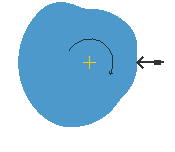
\includegraphics[width=0.9\textwidth]{part2/camme/FIG/camma/camma_punteria.pdf}}
\hfill
%\hspace{\fill}
\begin{picture}(0,0)(150,0)
\scriptsize{
\put(0,150){${\rho_0}_{\rm min}=46\; {\rm mm,\;}\;\alpha=126^{\circ}$}
\put(9,144){\rotatebox{-54}{$\longrightarrow$}}
\put(39,145){\rotatebox{-77}{$\longrightarrow$}}
\put(43,140){$\theta_{\rm max}=35^{\circ},\; \alpha=103^{\circ}$}
}
\end{picture}
      \caption{\em Camma tastata da una punta, $R_b=80\;{\rm mm}$.}
 \label{fig:f_camma_punteria}
\end{minipage}
\hfill
\begin{minipage}[b]{0.46\textwidth}
\centering
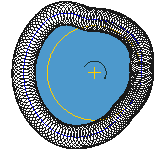
\includegraphics[width=0.9\textwidth]{part2/camme/FIG/camma/inviluppo.pdf}
\begin{picture}(0,0)(148,-2)
\scriptsize{
\put(5,135){${\rho}_{\rm min}=26\; {\rm mm,\;}\;\alpha=126^{\circ}$}
\put(49,99){\rotatebox{-234}{$\longrightarrow$}}
\put(41.5,85.2){\rotatebox{-112}{\color{yellow}$\scriptscriptstyle{\rm circ}$}}
\put(40.9,74.9){\rotatebox{-94.5}{\color{yellow}$\scriptscriptstyle{\rm onf}$}}
\put(40.7,65){\rotatebox{-81}{$\color{yellow}\scriptscriptstyle{\rm ere}$}}
\put(42,56.5){\rotatebox{-70}{\color{yellow}$\scriptscriptstyle{\rm nza}$}}
\put(46,46){\rotatebox{-55}{\color{yellow}$\scriptscriptstyle{\rm di}$}}
\put(50.5,39.7){\rotatebox{-39}{\color{yellow}$\scriptscriptstyle{\rm  base}$}}
}
\end{picture}
      \caption{\em Profilo della camma inviluppato dal moto relativo della rotella di raggio  $r_r=20\; {\rm mm}$.}
     \label{fig:f_inviluppo}
\end{minipage}
\end{figure}
\noindent In figura \ref{fig:f_inviluppo} viene riportata la camma con il suo profilo
effettivo ottenuto dall'inviluppo
della rotella il cui centro segue il tracciato blu sul quale \`e posizionata,
cio\`e il {\em profilo del centro rotella}\index{profilo centro rotella}.
\noindent Le figure \ref{fig:f_camma_punteria} e \ref{fig:f_inviluppo} evidenziano un'altra
grandezza di elevato
rilievo nel progetto di una camma: 
la {\em curvatura}\index{curvatura!del profilo} del suo profilo.
Nelle due figure appena citate sono infatti riportati i valori minimi
di $\rho_0(\alpha)$ e $\rho(\alpha)$, che sono rispettivamente il raggio di curvatura
del profilo seguito dal centro della rotella e il raggio di curvatura del profilo fisico
della camma, valori variabili ovviamente da punto a punto.
Come nel caso dell'angolo di pressione, anche il controllo del raggio di curvatura \`e
di importanza fondamentale durante la fase di progetto.
Il profilo inviluppato dalla rotella, cio\`e l'effettivo profilo
della camma, presenter\`a raggi di curvatura  che saranno dati da $\rho=\rho_0-r_r$,
dove $r_r$ rappresenta il raggio della rotella stessa. \`E chiaro quindi che  
il raggio di curvatura del profilo effettivo pu\`o diventare
nullo o persino negativo nel caso in cui il raggio della rotella sia maggiore 
del minimo raggio di curvatura delle zone convesse 
del profilo del centro rotella.
Perci\`o, valori di $\rho_0$ eccessivamente bassi, nei tratti convessi di
tale profilo, possono causare le situazioni di {\em sottotaglio}\index{sottotaglio}
rappresentate in figura \ref{fig:f_sottotaglio},
e contrassegnate con le lettere $A$ e $B$. In tali zone si verifica che l'inviluppo
generato dalla rotella porta a un profilo intrecciato a coda di rondine,
quindi impossibile da seguire con un normale cedente.
\begin{figure}[t]
\hbox{
\vspace{-2cm} \hspace{.6cm}

\includegraphics[width=0.3\textwidth]{part2/camme/FIG/camma/sottotaglio_dettaglio.pdf}
}
%\rule[-4cm]{5pt}{6cm}
\hspace{-6cm}
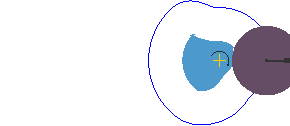
\includegraphics[width=1.4\textwidth]{part2/camme/FIG/camma/sottotaglio.pdf}

\begin{picture}(0,0)(-100,0)
\scriptsize{
\put(-31,245){A}
\put(64.5,175){A}
\put(137,154){B}
}
\end{picture}
      \caption{\em Camma con evidente sottotaglio, raggio rotella $r_r=58\;{\rm mm}$.}
     \label{fig:f_sottotaglio}
\end{figure}
\noindent Va per\`o detto che occorre tenere il valore di ${\rho}_{\rm min}$
ben lontano anche dallo zero, cio\`e dallo spigolo vivo che si verificherebbe
se il centro della rotella seguisse  una curva di raggio uguale a quello della rotella stessa.
La trasmissione delle forze, a volte ingenti, tra camma e punteria a rotella si basa
sul contatto tra una generatrice del ``cilindroide'' della camma e una del
cilindro della rotella stessa. Le pressioni di contatto che si generano in questi casi
si possono ricavare dalla {\em teoria di Hertz} per i contatti tra solidi elastici.
In particolare, nel nostro caso il contatto avviene tra due cilindri aventi raggio
$\rho$ per la camma e $r_r$ per la rotella, quindi possiamo affermare che la pressione di contatto
$p_c$ sar\`a \cite{timoshenko}, pagg. 418-419\footnote{Questo testo ha rappresentato per  
molto tempo un utile riferimento per tutti i problemi inerenti
il comportamento elastico dei solidi.},
\begin{equation}
p_c \propto \sqrt {{\rho + r_r}\over {\rho r_r}}\,,
\label{eq_hertz}
\end{equation}
\noindent che esplicita la proporzionalit\`a inversa tra tale pressione e la radice
quadrata del prodotto dei due raggi. Risulta quindi chiaro che il desiderio
di non far nascere pressioni troppo elevate, le quali potrebbero compromettere
la forma della
camma deformandola plasticamente, ci porta a desiderare un raggio minimo per il
profilo percorso dalla rotella ben lontano dallo zero
(lo spigolo). Raramente si progettano camme in cui si trovi nelle convessit\`a
del profilo un raggio minore alla met\`a di quello della rotella che lo tasta.
A questo proposito, mostriamo in figura \ref{fig:f_camma_rotella} una camma
correttamente profilata, la quale rappresenta con pi\`u
dettagli la stessa di figura \ref{fig:f_inviluppo}. Si nota che il valore dell'angolo
di pressione massimo non cambia rispetto alla situazione di cedente a punta,
\cite{molian}, pag. 61,
e il raggio minimo di curvatura del profilo risulta
accettabile.
Anche qui, come abbiamo fatto per l'angolo di pressione, ci si potrebbe incamminare alla ricerca
del legame che intercorre tra le leggi di moto, il raggio di base della camma, il raggio della rotella e  
il minimo raggio di curvatura (convessa) che si otterr\`a sul profilo.
Il volume \cite{ruggieri} riporta, a mio avviso, una delle pi\`u ampie e utili
trattazioni della sintesi di meccanismi a camma. Su questo libro si trova,
a pagina 59, una formula che lega il raggio del percorso del centro della rotella
con i valori del raggio di base, della salita $y(\alpha)$ e delle sue derivate, prima e seconda.
Si ha per il raggio del percorso del  ``centro rotella''\index{curvatura!formula}
\begin{equation}
\rho_0={{[{y'}^2+(R_b + y)^2]}^{3/2}\over{(R_b + y)^2-(R_b +y)y'' +2{y'}^2}}\,.
\label{r_cur}
\end{equation}
\noindent Pertanto elevati valori di accelerazione negativa generano raggi di curvatura modesti, come anche 
eccessivi valori per la velocit\`a $y'(\alpha)$, mentre, ancora una volta, a
un aumento del raggio di base $R_b$ corrisponde un aumento del raggio di curvatura
del profilo, ma come sempre anche un poco desiderabile aumento dell'ingombro. 
\begin{figure}[h]
\centering
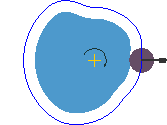
\includegraphics[width=0.9\textwidth]{part2/camme/FIG/camma/camma_rotella.pdf}
\begin{picture}(0,0)(235,-72)
\scriptsize{
\put(0,150){${\rho}_{\rm min}=26\; {\rm mm,\;}\;\alpha=126^{\circ}$}
\put(24,133){\rotatebox{126}{$\longrightarrow$}}
\put(69,124){\rotatebox{103}{$\longrightarrow$}}
\put(58,112){$\theta_{\rm max}=35^{\circ}, \alpha=103^{\circ}$}
}
\end{picture}
      \caption{\em Camma correttamente profilata, $R_b=80\, {\rm mm}$, $r_r=20\, {\rm mm}$.}
 \label{fig:f_camma_rotella}
\end{figure}
\noindent Nonostante ricavare la \ref{r_cur} non presenti difficolt\`a insormontabili, abbiamo
preferito evitare la sua  dimostrazione che sarebbe risultata lunghetta anzich\'e no,
e avrebbe aggiunto poco alla comprensione del problema che stiamo trattando.
\noindent Oggigiorno la profilatura delle camme si esegue totalmente
con tecniche numeriche e l'individuazione dei punti cospicui, cio\`e quelli che presentano il valore pi\`u elevato dell'angolo
di pressione e il minore raggio di curvatura, risulta essere piuttosto semplice:
normalmente i programmi di calcolo li rendono facilmente rintracciabili
evidenziandoli.
Le figure \ref{fig:ap_camma_rotella} e \ref{fig:cur_camma_rotella} dovrebbero
dare
l'idea della variazione delle due grandezze fondamentali, $\theta$ e $\rho$, per
la camma di figura \ref{fig:f_camma_rotella}. Mentre il grafico di
$\theta$ \`e contenuto entro precisi limiti, quello di $\rho$ pu\`o assumere
valori assoluti molto grandi ($\rho$ \`e infinito nei punti di flesso
del profilo), pertanto una parte di tale grafico \`e escluso dalla figura.
\begin{figure}[b]
\centering
\begin{minipage}[b]{0.48\textwidth}
\centering
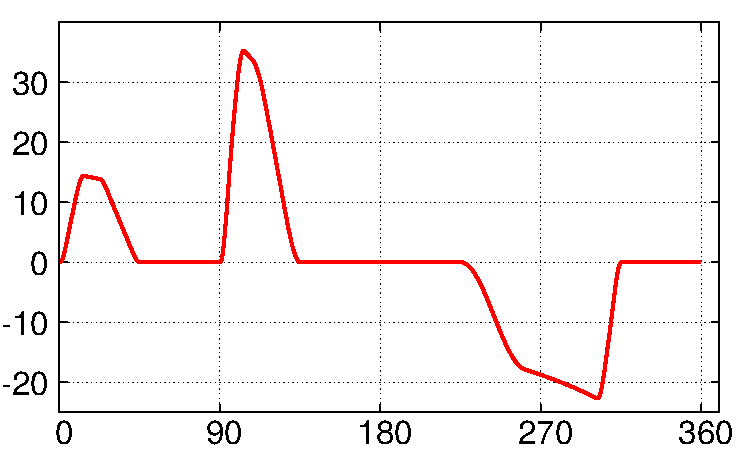
\includegraphics[width=0.9\textwidth]{part2/camme/FIG/camma/ck_ang_press_camma_punteria.pdf}
\begin{picture}(0,0)(130,0)
\scriptsize{
}
\put(127,2){$\alpha$}
\put(-31,86){$\theta$}
\end{picture}
      \caption{\em Andamento di $\theta$ per la camma di figura \ref{fig:f_camma_rotella}.}
 \label{fig:ap_camma_rotella}
\end{minipage}\hfill
\begin{minipage}[b]{0.48\textwidth}
\centering
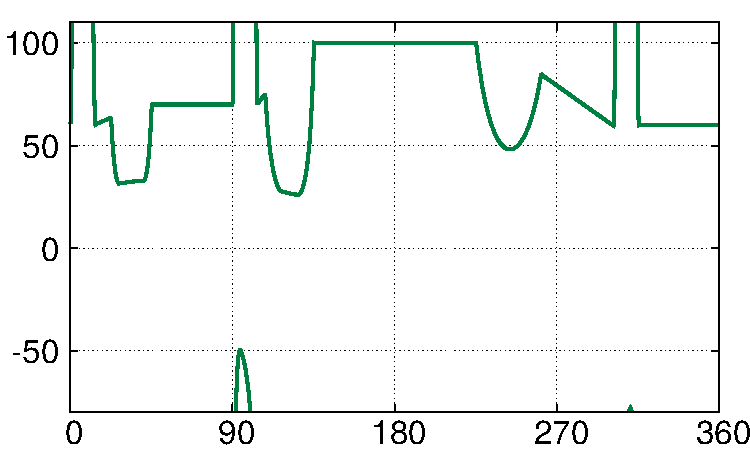
\includegraphics[width=0.9\textwidth]{part2/camme/FIG/camma/ck_cur_camma_rotella.pdf}
\begin{picture}(0,0)(129,0)
\scriptsize{
\put(127,2){$\alpha$}
\put(-38,86){$|\rho|$}
}
\end{picture}
      \caption{\em Andamento di $|\rho|$ per la camma di figura \ref{fig:f_camma_rotella}.}
     \label{fig:cur_camma_rotella}
\end{minipage}
\end{figure}
\noindent Mediante opportune maggiorazioni e minorazioni dei termini della
\ref{r_cur} si pu\`o ottenere, anche in questo caso, 
una formula di progetto per $R_b$, come mostrato in \cite{ruggieri}, pag. 72, formula che non riportiamo.
Aggiungiamo, tuttavia, qualche considerazione
qualitativa circa l'individuazione del raggio di base, mettendolo maggiormente
in luce nella \ref{r_cur}, riscrivendola nel seguente modo
\begin{equation}
\rho_0={{{{[{{y'}^2\over{(R_b + y)^2}}+1]}^{3/2}(R_b+y)}\over{{1-{y''\over{(R_b + y)}}} +{2{y'}^2\over{(R_b + y)^2}}}}}\,.
\label{r_cur1}
\end{equation}
\noindent Notiamo che, a un aumento del raggio di base $R_b$, il valore assoluto del 
termine del denominatore che contiene $y''$
diminuisce, e con esso
cala la possibilit\`a che il denominatore (nel caso di valori negativi di
$y''$) diventi troppo grande e tale da compromettere il 
raggio di curvatura della camma.
Ma soprattutto osserviamo una squisita ``quasi proporzionalit\`a''
tra $\rho_0$ e $R_b$ essendo $\rho_0\approxprop (R_b +y)$, la quale proporzionalit\`a ci garantisce che all'aumentare del raggio di base spariscono
i problemi legati a raggi di curvatura troppo piccoli del profilo.
Perci\`o, aumentando il raggio di base ci togliamo
sia dall'impaccio di angoli di pressione troppo elevati
sia dal pericolo di curvature eccessive del profilo della camma.


\noindent Nonostante la presenza di una formula che pu\`o guidarci
durante il progetto verso un valore di $R_b$ rispettoso dei limiti da imporre
alla curvatura,
la sintesi delle camme, come si \`e detto, si esegue sempre pi\`u spesso 
per tentativi ripetuti, mediante codici dedicati
che rendono veloce ed efficace il confronto tra soluzioni diverse: a un angolo di
pressione massimo troppo grande o a un raggio di curvatura del profilo eccessivamente
ridotto segue un nuovo tentativo con $R_b$ aumentato, oppure anche con modifiche
(tollerabili) alle leggi di moto.

\noindent Anche se in questa sede abbiamo ritenuto 
di fornire soltanto un'infarinatura generale che
renda chiari i concetti e le difficolt\`a che stanno alla base della progettazione
delle camme, in un perimetro di studi pi\`u vasto si trova qualche
altro ``trucco'' che permette
di non aumentare, oltre il ragionevole, l'ingombro di questi eccentrici e allo stesso
tempo di non eccedere coi valori dell'angolo di pressione. 
Uno di tali {\em escamotage} \`e quello di costruire un dispositivo camma-cedente in cui
l'asse di quest'ultimo non passi per il centro della camma stessa.
Il disassamento del cedente \`e in qualche modo equivalente a inclinare il cedente di un dato angolo che 
si sottrarr\`a all'angolo di pressione durante la salita, sommandosi invece a
questo nei tratti di discesa. Una discreta percentuale delle camme
che si realizzano sono di questo tipo: {\em camme a punteria deviata}\index{punteria deviata} oppure, con terminologia anglosassone,
{\em camme offset}\index{camme!offset}.
Un breve cenno alla progettazione di questi dispositivi si trova nel
capitolo di approfondimento \ref{cam2}.

\begin{figure}[b]
\centering
\begin{minipage}[b]{0.68\textwidth}
\centering
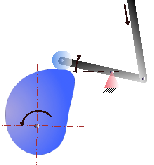
\includegraphics[width=0.9\textwidth]{part2/camme/FIG/cambil.pdf}
\begin{picture}(0,0)(150,-20)
\scriptsize{
}
\put(35,143){$\beta(t)$}
\put(-29,60){$\omega$}
\end{picture}
        \caption{\em Camma con cedente a bilanciere.}
     \label{fig:f_cambil}
\end{minipage}\hfill
\begin{minipage}[b]{0.28\textwidth}
\centering
     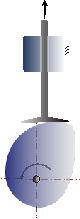
\includegraphics[width=0.9\textwidth]{part2/camme/FIG/campiat.pdf}
\begin{picture}(0,0)(70,-20)
\scriptsize{
}
\put(7,214){$y(t)$}
\put(10,45){$\omega$}
\end{picture}
        \caption{\em Camma tastata da un piattello.}
     \label{fig:f_campiat}
\end{minipage}\hfill
\end{figure}

\noindent Le camme possono azionare cedenti che non traslano, come mostrato
in figura \ref{fig:f_cambil}.
Sono diffusissimi meccanismi in
cui la camma impone al
cedente a bilanciere un moto rotatorio.
Mutando opportunamente
ci\`o che nel ragionamento si deve mutare e in particolare sostituendo l'alzata $y(t)$ con l'angolo
che descrive il bilanciere nella sua rotazione, $\beta(t)$, tutto quanto esposto circa le precauzioni
nel progetto della camma rimane invariato: le leggi di moto con i loro
 coefficienti di velocit\`a e di accelerazione si scelgono con gli stessi criteri e
nella profilatura della camma si devono fare i soliti conti con curvatura e angolo di 
pressione. Anche qui, rimandiamo il lettore desideroso di approfondire un poco la
progettazione delle camme tastate da cedente a bilanciere al capitolo
\ref{cam2}, oppure a \cite{ruggieri}, pag. 74.


\noindent La trasmissione del movimento tra camma e cedente non avviene sempre tramite il rotolamento
di una rotella sul profilo della camma. Bench\'e tastare una camma con un {\em piattello}\index{piattello}, come in figura \ref{fig:f_campiat}, sia ormai raro nell'ambito delle macchine automatiche, in altri 
domini della meccanica la soluzione camma-piattello \`e molto usata.
Anzi, a dire il vero, vi \`e un vastissimo repertorio di camme tastate esclusivamente
da piattelli che, strisciando sul profilo, in questo caso
rigorosamente convesso di quest'ultime,
aziona cedenti a punteria o a bilanciere: le camme dei motori endotermici a quattro
tempi. Si tratta in genere di camme di dimensioni modeste alle quali calza naturalmente
tutta la teoria qui esposta. 

\noindent Una breve introduzione alla progettazione
delle camme tastate da piattelli si trova nel capitolo di
approfondimento \ref{cam2} e, per esteso, in \cite{ruggieri}, pag. 65.
 I problemi legati alla progettazione di queste camme
sono per\`o di natura cos\`i
diversa da quelli che si incontrano nelle macchine automatiche, la loro progettazione
segue dettami cos\`i intimamente legati alla legge delle alzate, a sua volta legata
al percorso dei gas nei condotti fluidodinamici che esse aprono e chiudono, che
ci sembra meglio lasciare questi piccoli e sofisticati eccentrici al loro
mondo, cio\`e quello motoristico, e tornare alle nostre camme per macchine
automatiche.

\begin{figure}[t]
\centering
\begin{minipage}[b]{0.48\textwidth}
\centering
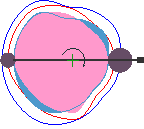
\includegraphics[width=0.9\textwidth]{part2/camme/FIG/camma/camma_desmo.pdf}
\begin{picture}(0,0)(130,0)
\scriptsize{
}
\end{picture}
      \caption{\em Camma desmodromica.}
 \label{fig:f_camma_desmo}
\end{minipage}\hfill
\begin{minipage}[b]{0.48\textwidth}
\centering
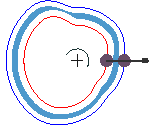
\includegraphics[width=0.9\textwidth]{part2/camme/FIG/camma/desmo_costola.pdf}
\begin{picture}(0,0)(129,0)
\scriptsize{
}
\end{picture}
      \caption{\em Camma a costola.}
     \label{fig:f_desmo_costola}
\end{minipage}
\end{figure}

\section{Camme Coniugate}

\noindent L'accoppiamento, cio\`e il contatto tra camma e cedente, pu\`o essere
 garantito nelle fasi di discesa\footnote{
Ribadiamo che il termine discesa si riferisce al movimento contrario
a quello generato dalla camma mentre compie il suo lavoro funzionale.
Esso non si riferisce
quindi in alcun modo all'avvicinamento alla Terra.
} in due diversi modi:
imponendo che la punteria prema sulla camma durante tutto l'angolo giro, oppure
facendo in modo, mediante una camma accoppiata a quella primaria, che la punteria
sia costretta a seguire il profilo di questa anche nei tratti che presentano $\dot y$ 
negative.
Nel primo caso si parla di {\em accoppiamento di forza}\index{accoppiamento!di forza}
e molto spesso tale forza viene esercitata da una molla (quasi sempre
pre-caricata) che, deformata
durante le fasi di salita, garantisce mediante la sua elasticit\`a il contatto
anche durante la discesa. Questa soluzione \`e raramente impiegata nell'ambito
delle macchine automatiche, l'autore non ne ha mai vedute (ma il mondo
\`e grande...), mentre trova largo impiego nelle piccole camme ad uso motoristico.
Nel secondo caso si impone il contatto mediante un {\em accoppiamento di forma}\index{accoppiamento!di forma}, cio\`e progettando una camma ``negativa'' detta
{\em camma coniugata}\index{camme!coniugata} o {\em camma desmodromica}\index{camme!desmodromica}, riportata in colore rosa
nella figura \ref{fig:f_camma_desmo}.
La generazione di questa camma potrebbe in linea di principio seguire il percorso
per la progettazione della camma ``primaria'' avendo, in questo caso, l'avvertenza di invertire i
segni delle leggi di moto. Di fatto, una volta disegnata la camma primaria,
baster\`a
considerare il prolungamento del cedente fino al luogo ove si desidera tastare 
la camma desmodromica e riportare una seconda rotella.

\begin{figure}[hbt]
\centering
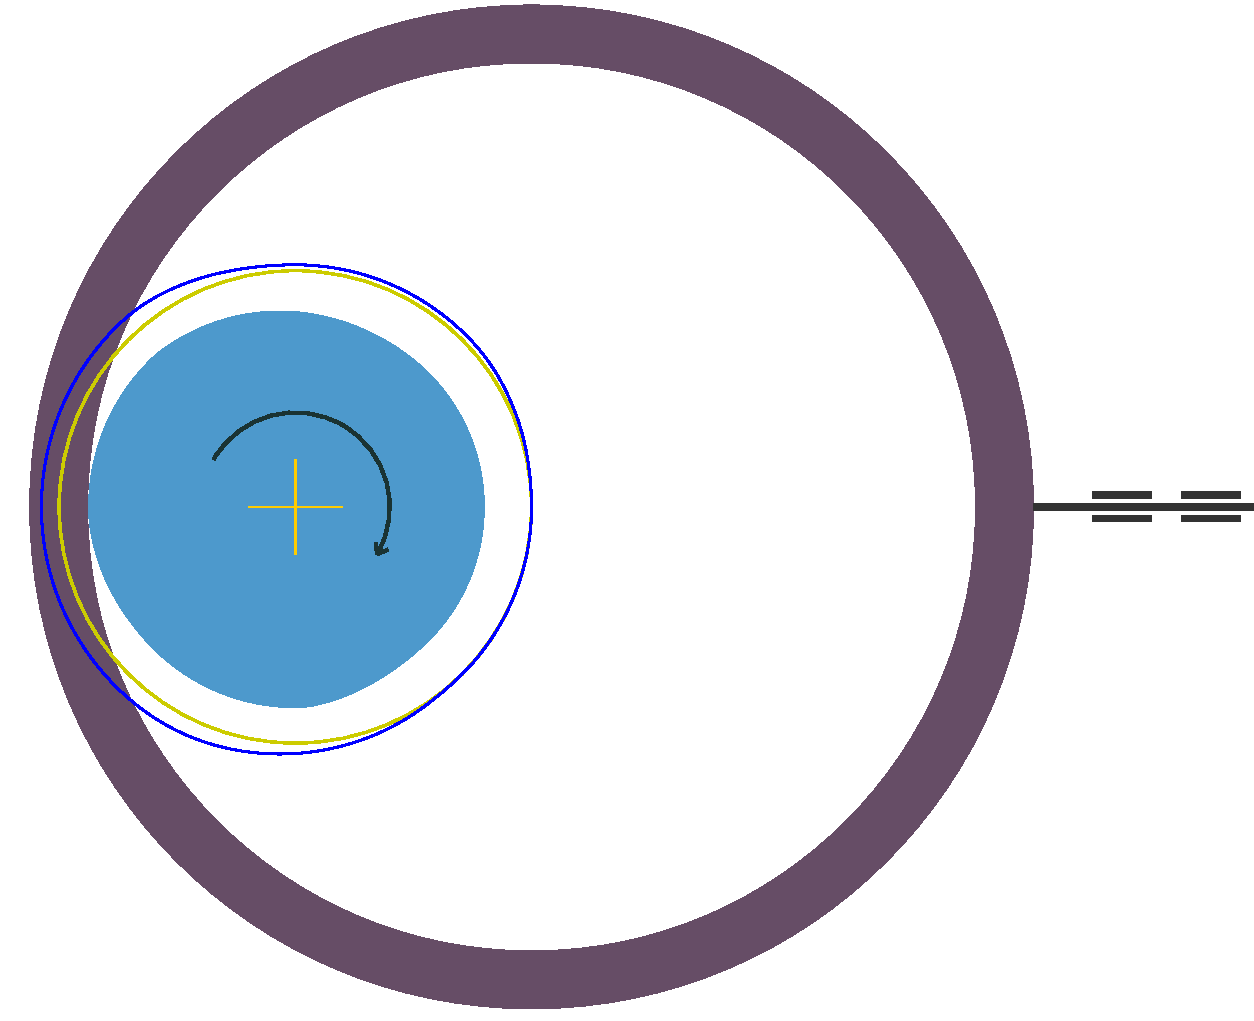
\includegraphics[width=0.85\textwidth]{part2/camme/FIG/camma/rotella_interna.pdf}
\begin{picture}(0,0)(130,0)
\scriptsize{
}
\end{picture}
      \caption{\em Camma tastata dall'anello interno di un cuscinetto.}
 \label{fig:f_rotella_interna}
\end{figure}


\noindent Tale 
rotella, durante il movimento generato dalla camma primaria (sottintendendo il contatto
costante tra cedente e profilo),  ``taglier\`a'' la camma desmodromica o {\em
camma coniugata}\index{camme!coniugata}, e questo modo di 
procedere \`e anche quello utilizzato dal nostro codice
per produrre le illustrazioni \ref{fig:f_camma_desmo} e 
\ref{fig:f_desmo_costola}. Delle due citate figure, la seconda rappresenta
una soluzione molto elegante di accoppiamento
desmodromico, dove le rotelle tastano una costola. Purtroppo, questa
soluzione non \`e
di facilissima realizzazione in officina. Normalmente le camme coniugate
sono pi\`u sottili delle relative primarie e le loro rotelle sono di
minori dimensioni.
Questo \`e dovuto alla funzione ``di servizio'' da loro svolta,
che semplicemente consiste nel mantenere il contatto tra la punteria e la
camma primaria
e nel riportare il cedente nella posizione di partenza: esse
svolgono molto raramente azioni di lavoro. Persino le cautele sull'angolo di
pressione massimo e sul minimo raggio di curvatura convessa,
ammesse per queste camme 
(parliamo sempre delle fasi attive), possono essere leggermente rilassate.

\noindent Anche la fantasia pu\`o partecipare con successo nella progettazione delle camme.
Riportiamo, in figura \ref{fig:f_rotella_interna}, 
una soluzione poco comune di camma-punteria dove
il profilo della camma viene tastato dall'anello interno di un cuscinetto
(a rulli). In tale figura, il meccanismo viene rappresentato nel momento in
cui la camma ha svolto $180^{\circ}$ della sua rotazione e, stanti le leggi
proposte per questa camma, la punteria si trova alla massima estensione 
dell'alzata.
Le due curvature, quella della camma e quella della rotella,
sono, in questo caso, concordi. Pertanto,
nella \ref{eq_hertz} uno dei due
raggi cambia segno e la pressione andrebbe addirittura
ad annullarsi nel caso (da non contemplarsi) di raggi di curvatura
uguali tra loro.
\begin{figure}[hbt]
\centering
\begin{minipage}[b]{0.48\textwidth}
\centering
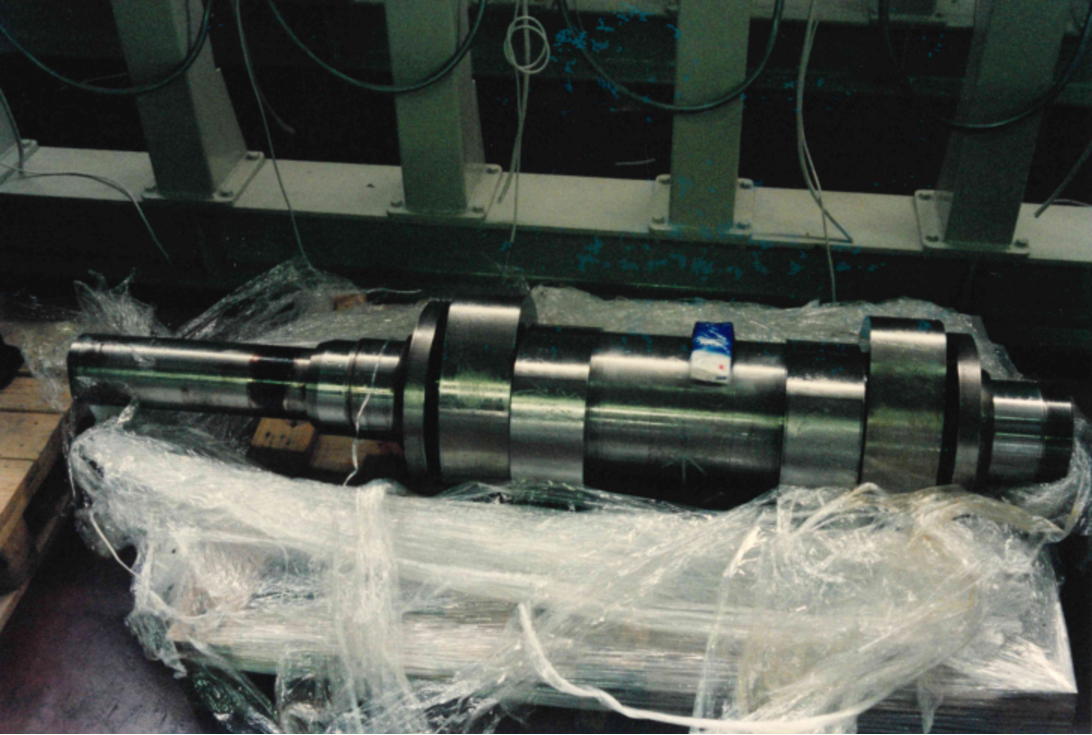
\includegraphics[width=0.9\textwidth]{part2/camme/FIG/albero.pdf}
\begin{picture}(0,0)(130,0)
\scriptsize{
}
\end{picture}
      \caption{\em Albero a camme per pressa di grandi dimensioni, tastato dall'anello interno di un cuscinetto.}
 \label{fig:f_albero}
\end{minipage}\hfill
\begin{minipage}[b]{0.48\textwidth}
\centering
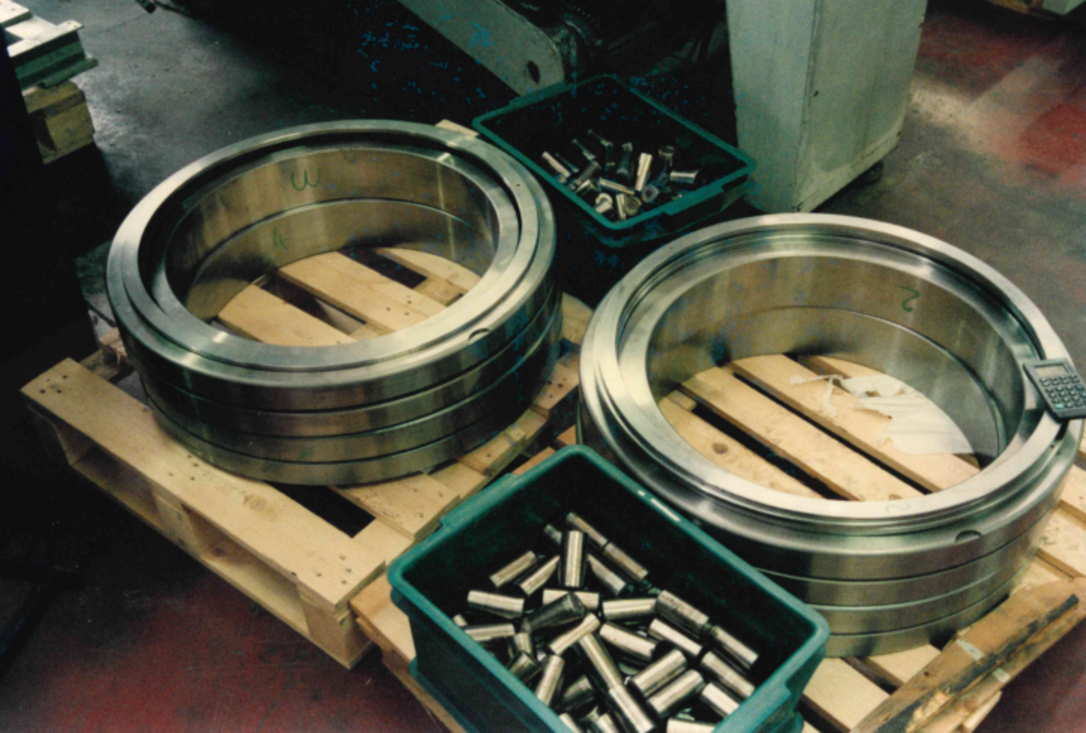
\includegraphics[width=0.9\textwidth]{part2/camme/FIG/rotella.pdf}
\begin{picture}(0,0)(129,0)
\scriptsize{
}
\end{picture}
      \caption{\em Rotella costituita da cuscinetto a rulli che tasta la camma mediante il suo anello interno.}
     \label{fig:f_rotella}
\end{minipage}
\end{figure}
\noindent La pressione di contatto risulta quindi
notevolmente ridotta in questo tipo di camme che possono essere usate quando le forze da trasmettere 
sono ingenti. Nelle figure \ref{fig:f_albero} e \ref{fig:f_rotella} riportiamo una realizzazione
della tipologia di camme appena descritte e di una delle quattro rotelle,
con il desiderio di mostrare al lettore quali ragguardevoli 
dimensioni possono essere raggiunte da un albero a camme e da una rotella.

\endinput
